\scanpage{19}
\mspage{8}
\margin{18}

$\operatorname{Pol}(D)$, en autant de sommets que l'indique son poids, on trouve un nouveau polygône combinatoire \inserted{$\widehat P(\Delta)$}, d'ordre $2(n-1)$, semblable à celui découpé par les $\Delta_i$ ($i\ne i_0$) sur une \uline{parallèle} à $\Delta$. Et on trouve une bijection canonique
\[
\widetilde{I\setminus\{i_0\}}\simeq\text{ens des \uline{sommets} de }\widehat P(\Delta_{i_0})
\]
compatible avec les antipodies.

\margin{NB Cette bijection dépend du choix d'une orientation de $\Delta_{i_0}$ --- en le changeant, on trouve la précédente composée avec l'antipodisme.}

\deleted{\figure{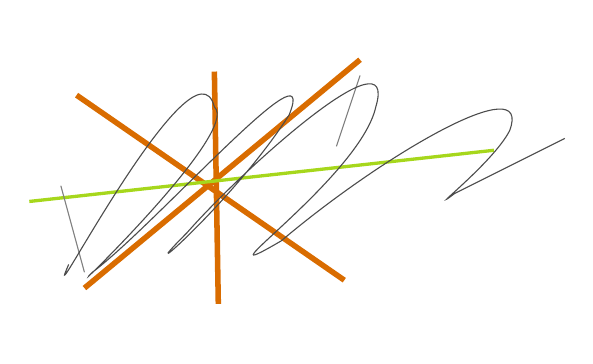
\begin{tikzpicture}[x=1cm,y=1cm]
\draw[orange!85!black,line width=2pt] (-1.7,-1.3)--(1.8,1.6) (-1.8,1.15)--(1.6,-1.2) (0,-1.5)--(-.05,1.45);
\draw[yellow!65!green,line width=1.2pt] (-2.4,-.2)--(3.5,.45);
\draw[gray,thin] (-1.7,-1.1)--(-2,0) (1.5,.5)--(1.8,1.4);
\draw[black!70] (-1.9,-1)..controls(-2.3,-1.9)and(-.3,2)..(-.05,1)..controls(.3,.7)and(-2,-1.5)..(-1.6,-1.1)..controls(-.8,-.5)and(1.3,1.9)..(.9,.9)..controls(.2,-.2)and(-1.2,-1.4)..(-.4,-.6)..controls(.3,.2)and(2.3,2)..(2,1)..controls(1.8,.1)and(-.4,-1.4)..(.8,-.7)..controls(2.1,.4)and(4,1.5)..(3.7,.7)..controls(3.5,.3)and(2.6,-.4)..(3,-.1)--(4.4,.6);
\end{tikzpicture}}}

\figure{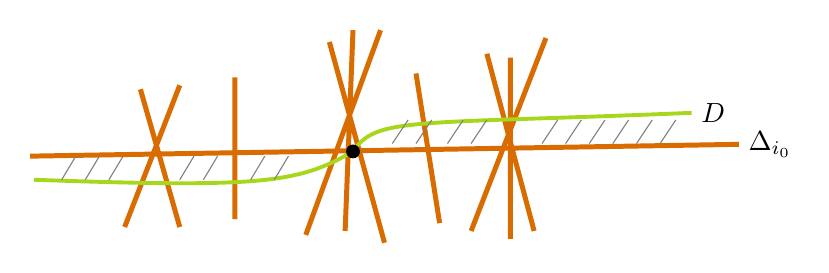
\begin{tikzpicture}[x=1cm,y=1cm]
\draw[orange!85!black,line width=1.8pt] (0,0)--(9,.15);
\draw[orange!85!black,line width=1.8pt] (1.2,-.9)--(1.9,.9) (1.9,-.9)--(1.4,.85) (2.6,-.8)--(2.6,1) (3.5,-1)--(4.45,1.6) (4,-.95)--(4.1,1.6) (4.5,-1.1)--(3.8,1.45) (5.2,-.85)--(4.9,1.05) (6.1,-1.05)--(6.1,1.25) (5.6,-.95)--(6.55,1.5) (6.4,-.95)--(5.8,1.3);
\draw[yellow!65!green,line width=1.4pt] (.05,-.3)..controls(2.9,-.4)and(3.4,-.35)..(4.1,.06)..controls(4.4,.5)and(4.8,.4)..(8.4,.55);
\foreach \x in {.4,.7,1,1.9,2.2,2.8,3.1}{\draw[gray,thin] (\x,-.3)--+( .18,.3);}
\foreach \x in {4.6,4.9,5.3,5.6,6.5,6.8,7.1,7.4,7.7,8}{\draw[gray,thin] (\x,.16)--+(.2,.3);}
\fill (4.1,.06) circle (2.5pt);
\node[right] at (8.4,.55) {$D$};\node[right] at (9,.15) {$\Delta_{i_0}$};
\end{tikzpicture}}

On aimerait comparer la pondération modifiée d'une arête en $\Delta$, avec sa pondération ordinaire. On trouve pour la pondération ordinaire $\nu_0$
\[
\begin{aligned}
\nu_0&=\text{Nb d'arêtes découpées sur la \unsure{ligne} $\unsure{D|\Delta}$ par $\Sigma$ le long}\\
&\qquad\text{du couloir}=\text{nb d'arêtes en }D=\deleted{\unsure{\operatorname{Card}(S\cap D)}}\ n-\nu.
\end{aligned}
\]
donc
\[
\nu+\nu_0=n
\]
donc la pondération modifiée résulte de la pondération ordinaire (si on connaît $n$. --- mais $n$ est déduit de la pondération ordinaire par les formules locales $\sum\text{de toutes les pondérations en }D=2n$ (où $D$ est un sommet non supercritique, p.ex. stable).

\deleted{\unsure{A}} On a ainsi trouvé une application canonique
\diagram{\begin{tikzcd}[ampersand replacement=\&,column sep=large]
\underbrace{\text{Sommets de }\Gamma(\underline\Sigma)}_{(=\operatorname{Pr}(\underline\Sigma))}\setminus\underbrace{\Sigma}_{\substack{\text{p.r. super}\\\text{critiques}}} \arrow[r] \& \substack{\text{ens des structures}\\\text{polygonales sur }\widetilde I\\\text{compatibles avec l'antipodisme,}}
\end{tikzcd}}
et il ne devrait pas être difficile de montrer que cette application est \uline{injective}. Il faudrait de plus, pour bien faire, voir :

1) Comment ``varient'' les $P(\unsure{D|\Delta})$, $\widehat P(\unsure{D|\Delta})$ le long d'une flèche de spécialisation,
